\documentclass[class=../report, crop=false]{standalone}
\usepackage{graphicx}
\usepackage{float}

\begin{document}

\section{Concepts Generated} \label{app:concepts}

\begin{figure}[H]
	\centering
	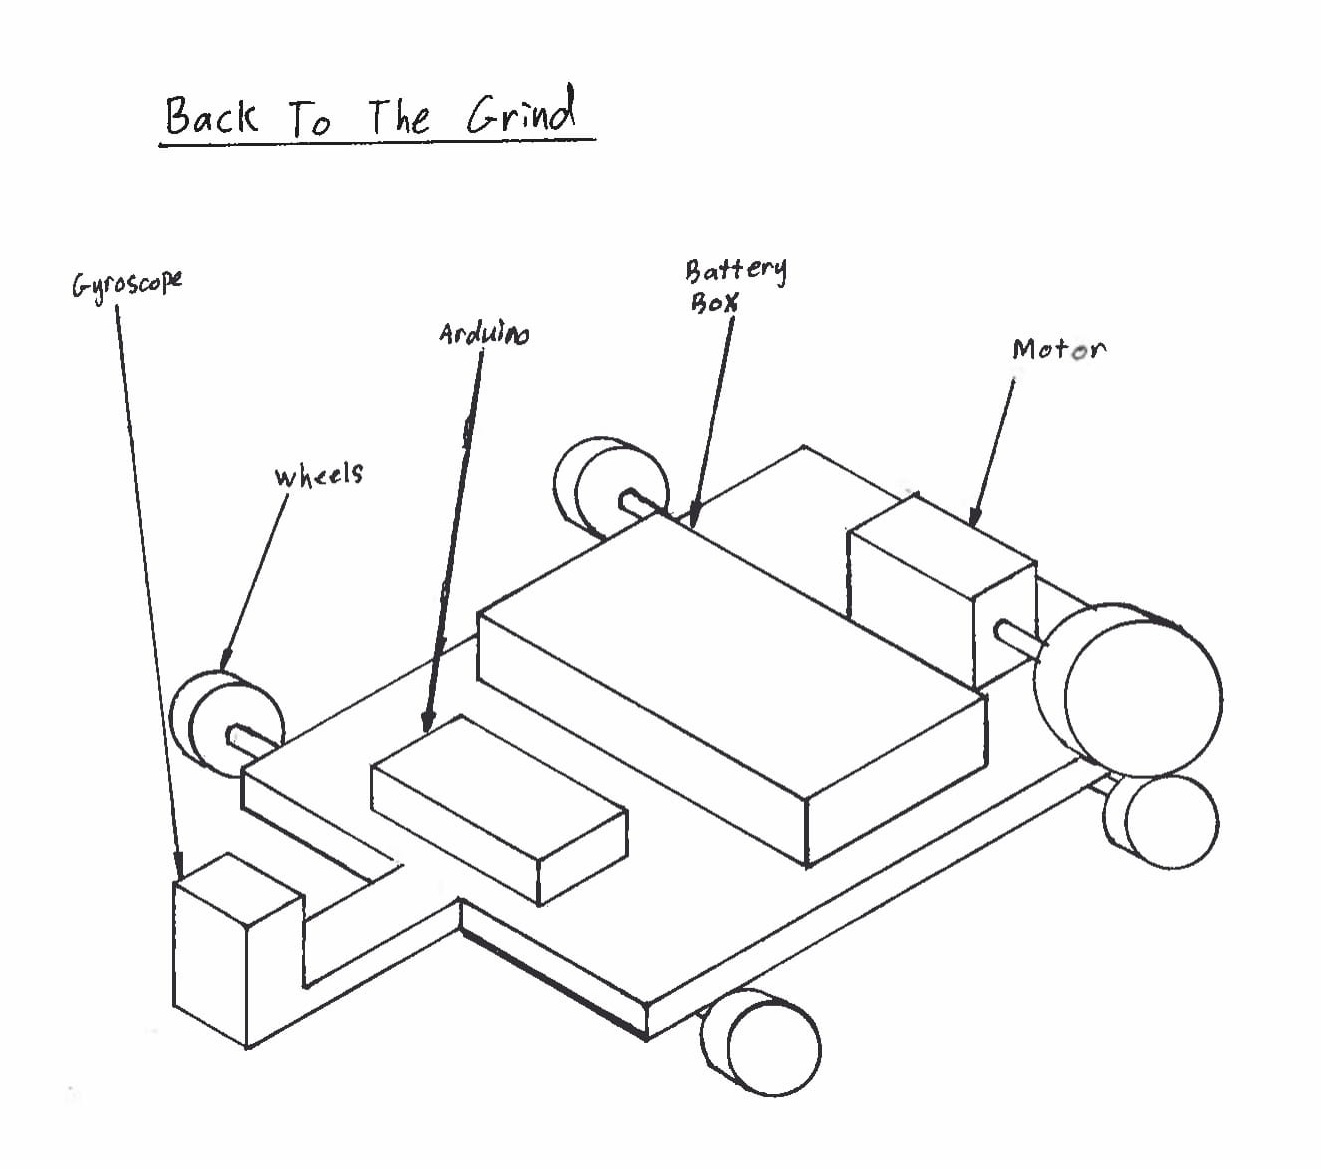
\includegraphics[width=0.8\textwidth]{../../res/img/bttg}
	\caption{Back to the Grind Concept Sketch}
	\label{app/fig:bttg}
\end{figure}

Description: Back to the Grind is a friction drive locomotive; as the motor directly transmits power to the rim of the back wheel.
The gyroscope reads the position and signals the Arduino when entering a turn; the motor then reverses, which causes the vehicle to brake.

\clearpage

\begin{figure}[H]
	\centering
	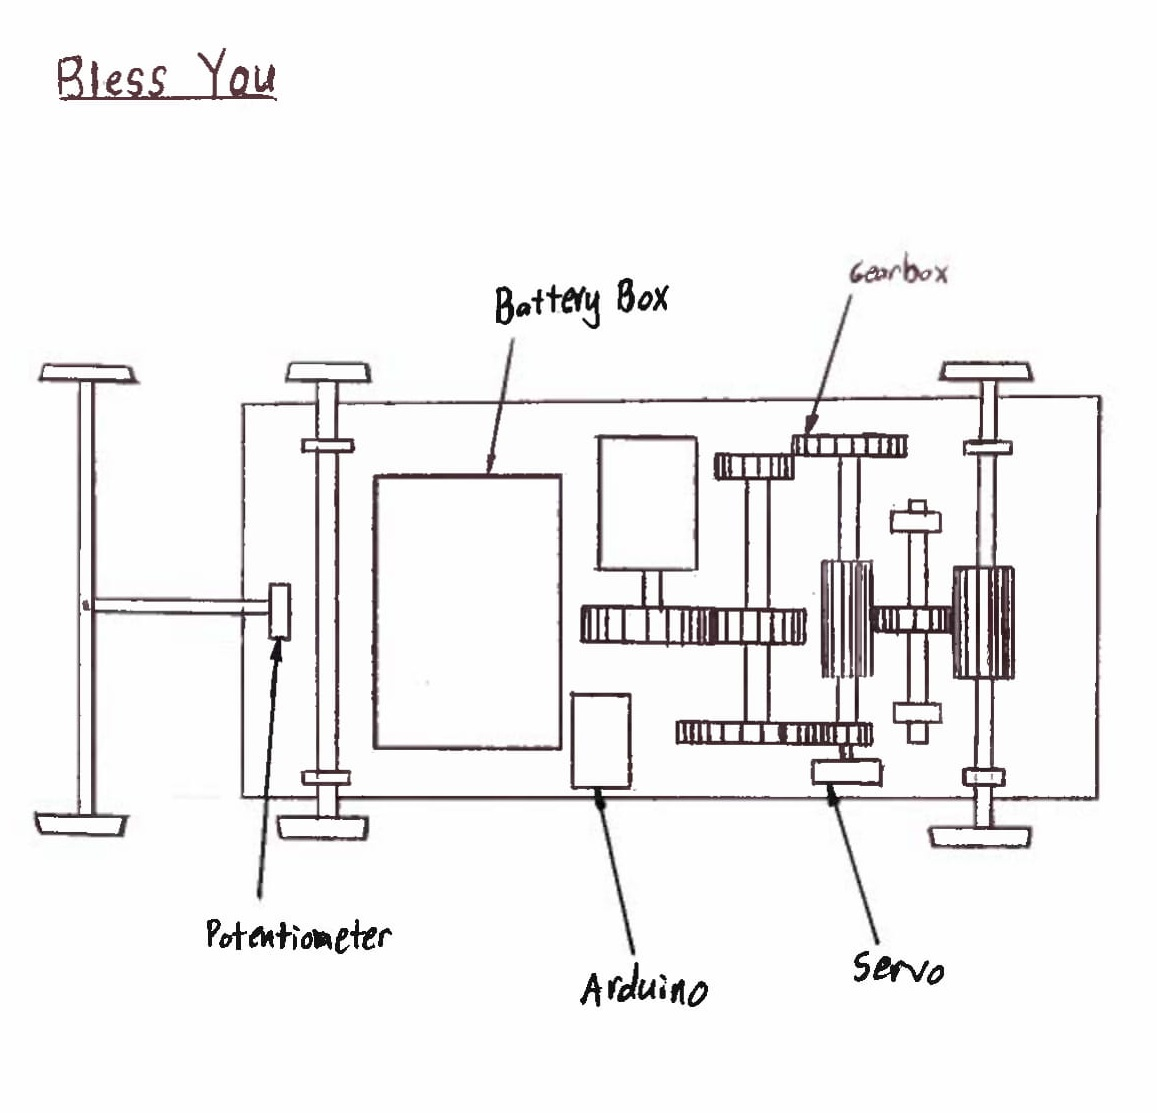
\includegraphics[width=0.8\textwidth]{../../res/img/blessyou}
	\caption{Bless You Concept Sketch}
	\label{app/fig:blessyou}
\end{figure}

Description: A design which uses a gearbox to control speed.
Wheels in front of the vehicle turn a potentiometer to detect turns.
When a turn is detected the Arduino will signal the motor to run in reverse.
Conical wheels will help with cornering.

\clearpage

\begin{figure}[H]
	\centering
	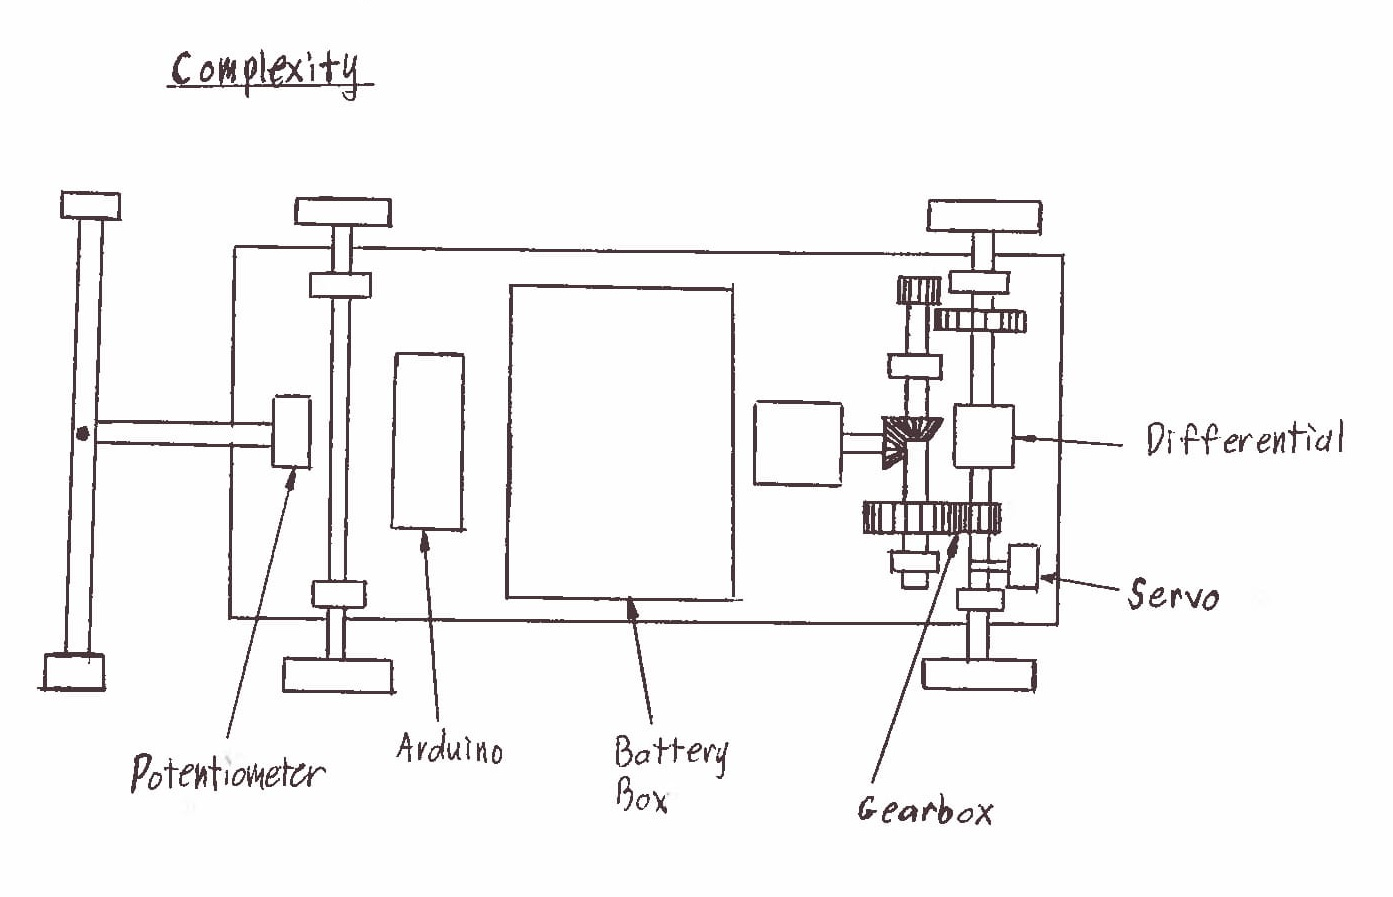
\includegraphics[width=0.8\textwidth]{../../res/img/complexity}
	\caption{Complexity Concept Sketch}
	\label{app/fig:complexity}
\end{figure}

Description: A design using a variable gearbox with dual speed and a differential to enable smoother turning.
Complexity uses a potentiometer on forward wheels in order to detect turns and slow down.

\clearpage

\begin{figure}[H]
	\centering
	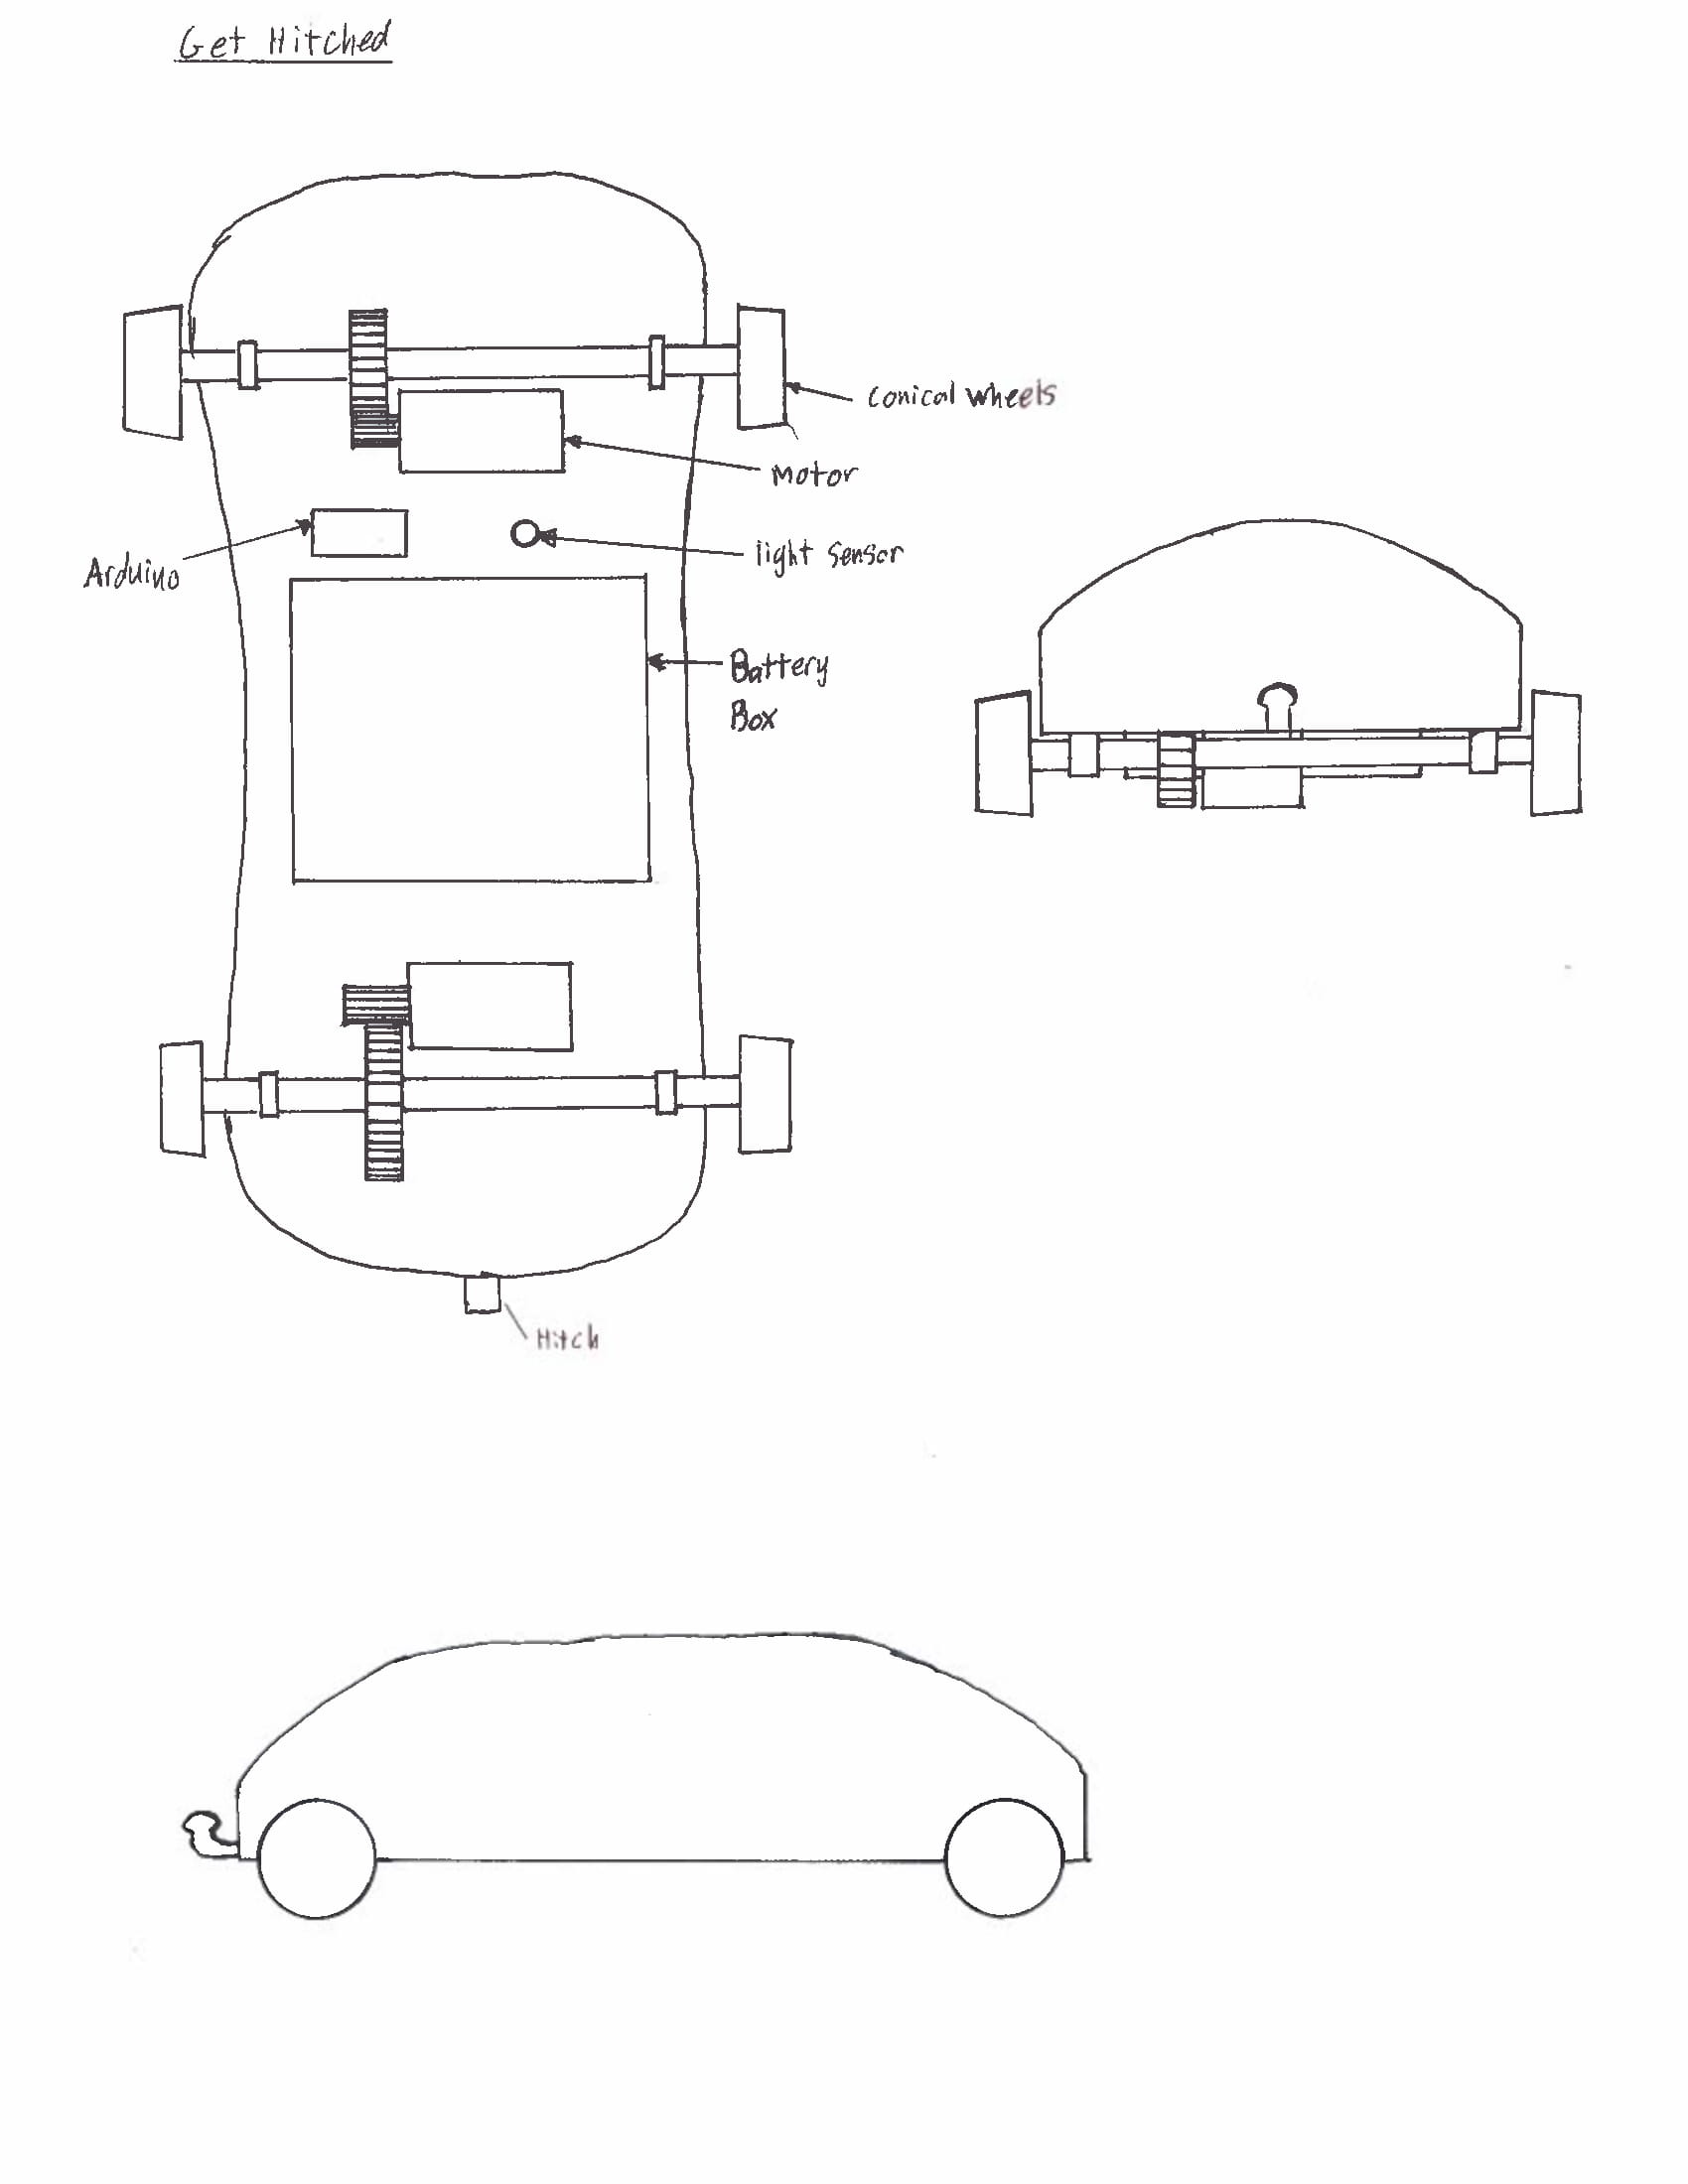
\includegraphics[width=0.8\textwidth]{../../res/img/gethitched}
	\caption{Complexity Concept Sketch}
	\label{app/fig:gethitched}
\end{figure}

Description: Get Hitched is a four wheel drive vehicle powered by two DC motors.
The design involves conical wheels for cornering and a light sensor that counts the rails in order to detect turns.

\clearpage

\begin{figure}[H]
	\centering
	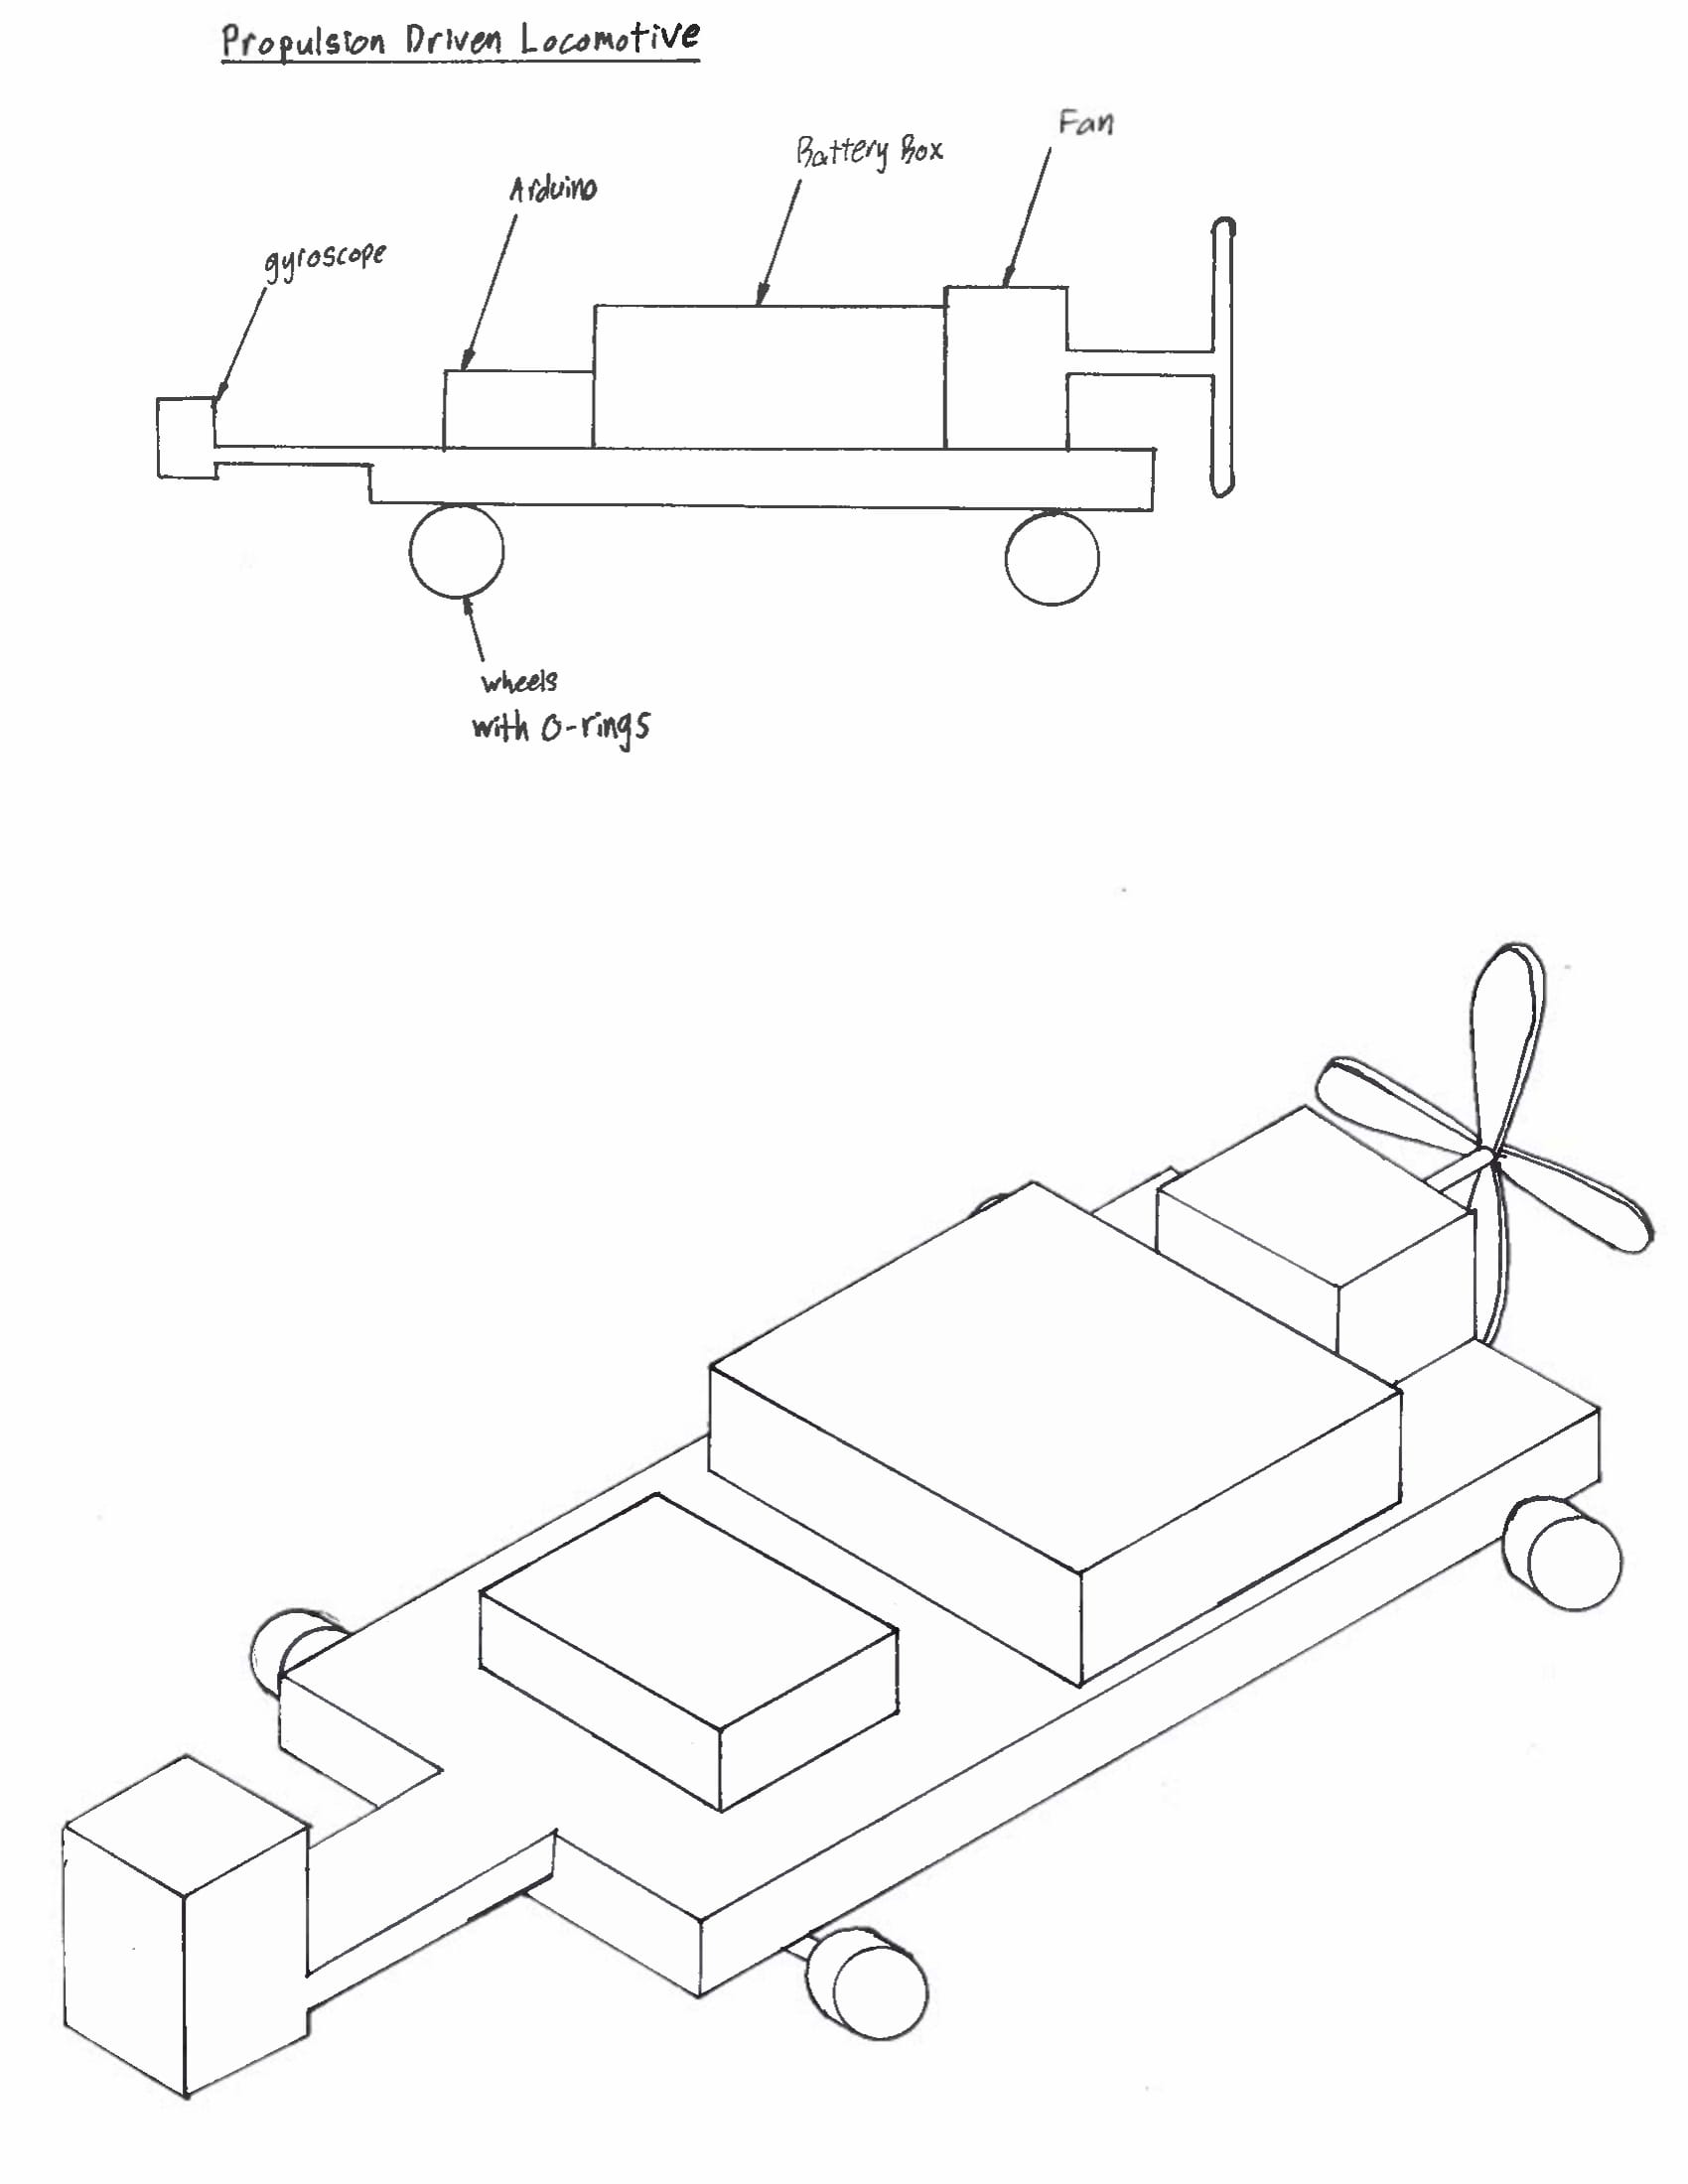
\includegraphics[width=0.8\textwidth]{../../res/img/pdl}
	\caption{Propulsion Driven Locomotive Concept Sketch}
	\label{app/fig:pdl}
\end{figure}


Description: The motor directly powers a fan that propels the locomotive.
The gyroscope coupled with the Arduino detect turns and lower the voltage on the fan to slow down.
The wheels in this design use o-rings in grooves to increase traction.

\clearpage

\begin{figure}[H]
	\centering
	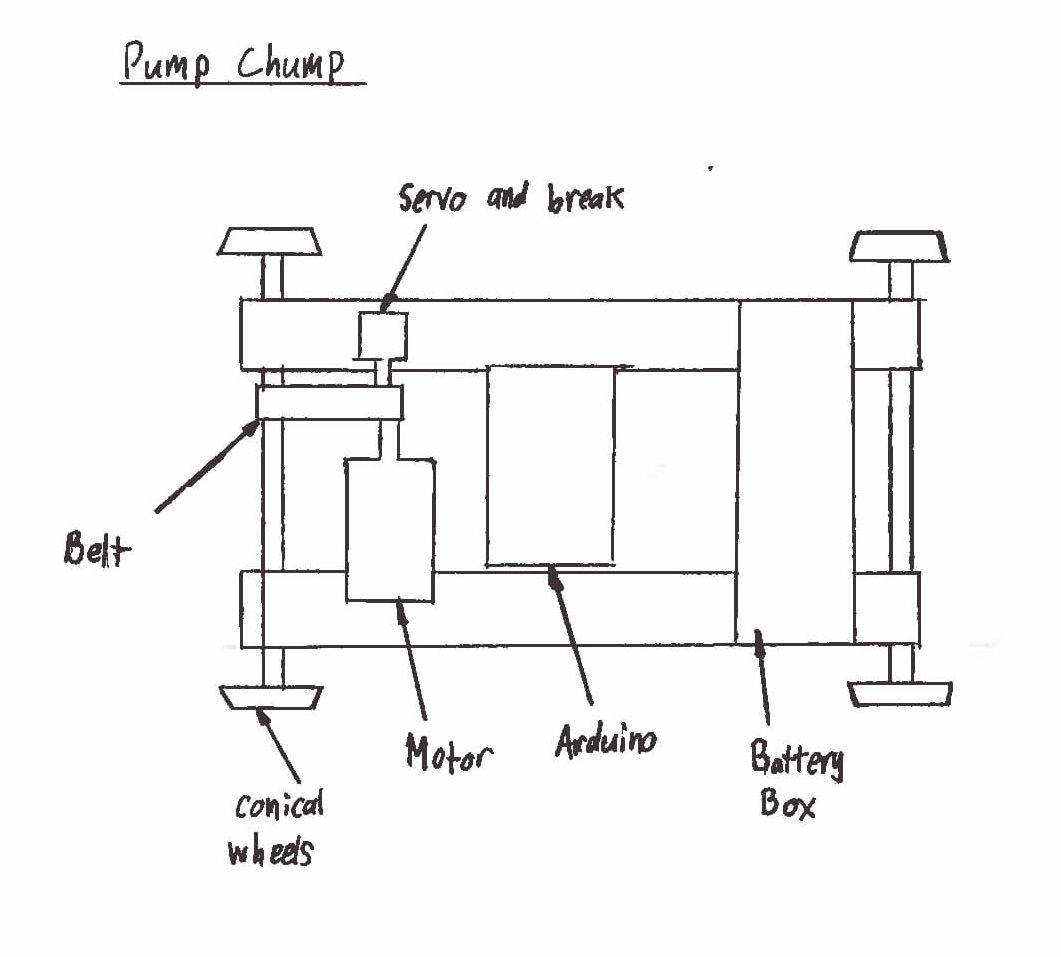
\includegraphics[width=0.8\textwidth]{../../res/img/pumpchump}
	\caption{Pump Chump Concept Sketch}
	\label{app/fig:pumpchump}
\end{figure}

Description: Pump Chump uses a belt drive for propulsion and brakes to control speed.
The Arduino is pre-programmed with track data and controls the motor and brakes.
This design uses conical wheels for cornering.
\clearpage

\begin{figure}[H]
	\centering
	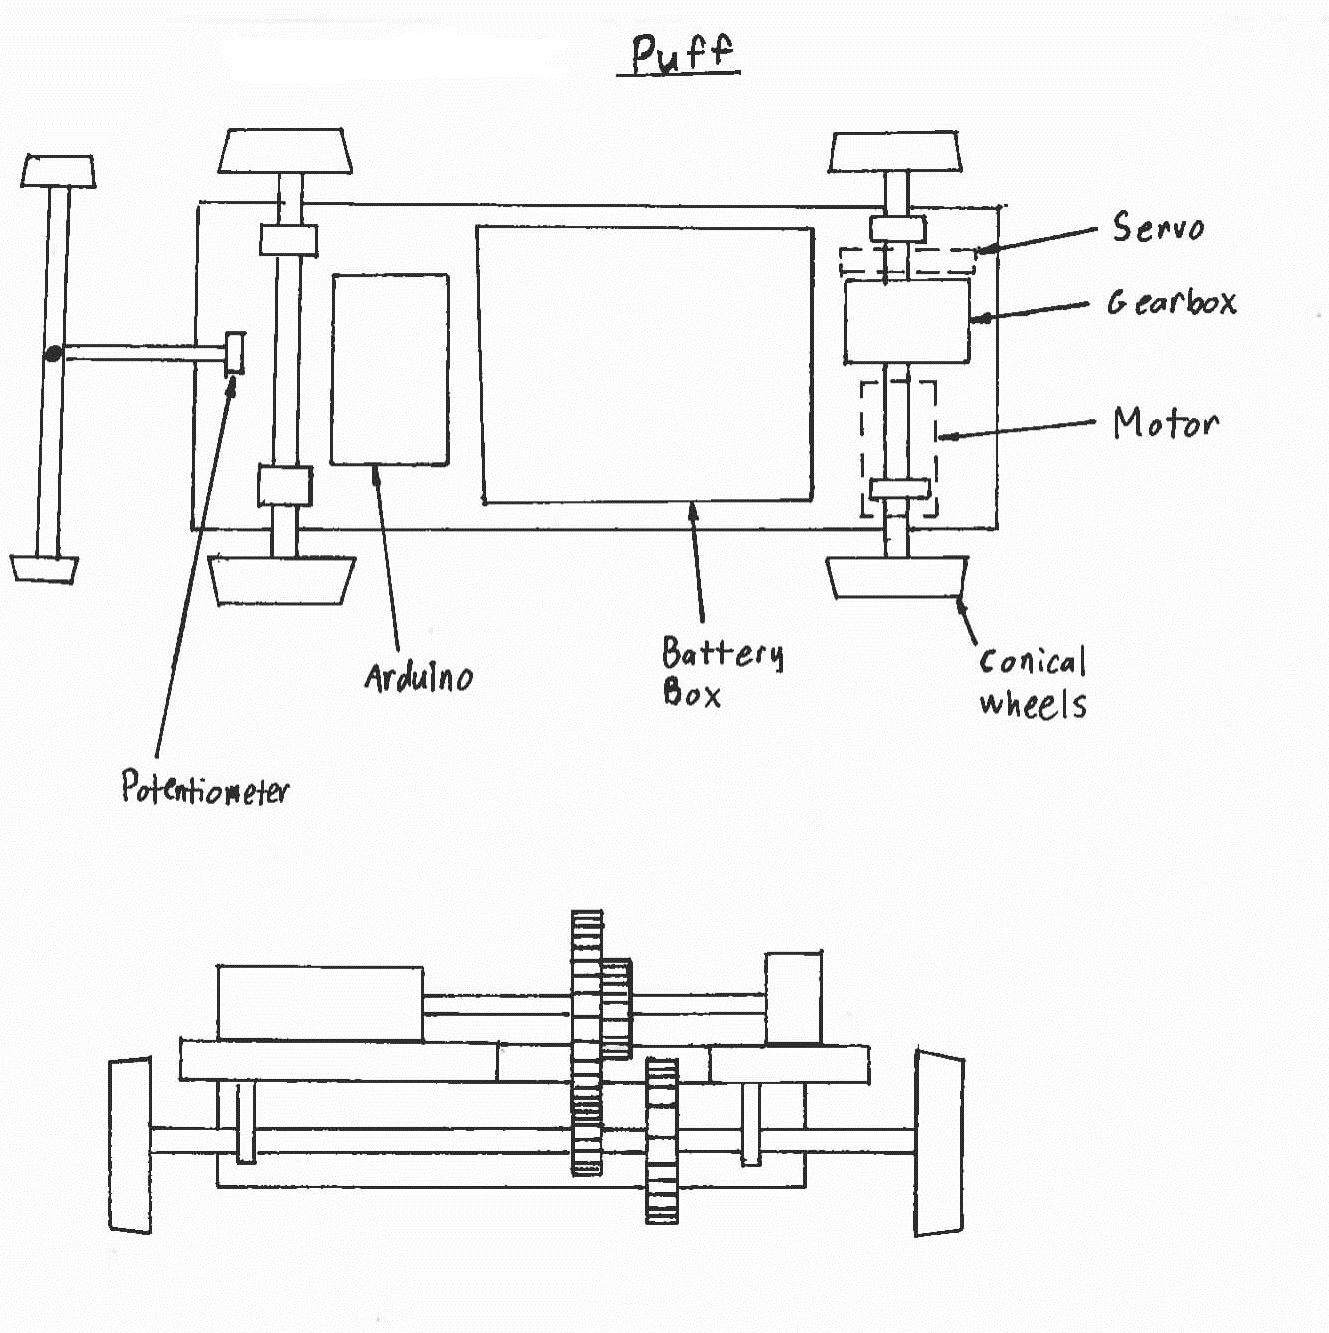
\includegraphics[width=0.8\textwidth]{../../res/img/puff}
	\caption{Puff Concept Sketch}
	\label{app/fig:puff}
\end{figure}

Description: Puff is a rear drive locomotive with a dual speed gearbox and conical wheels.
The servo switches the gears, rendering this design  an automatic gear shift mechanism.
Puff also involves a potentiometer that senses turns on the front wheels and transmits a signal to the arduino in order to slow down.
\clearpage

\begin{figure}[H]
	\centering
	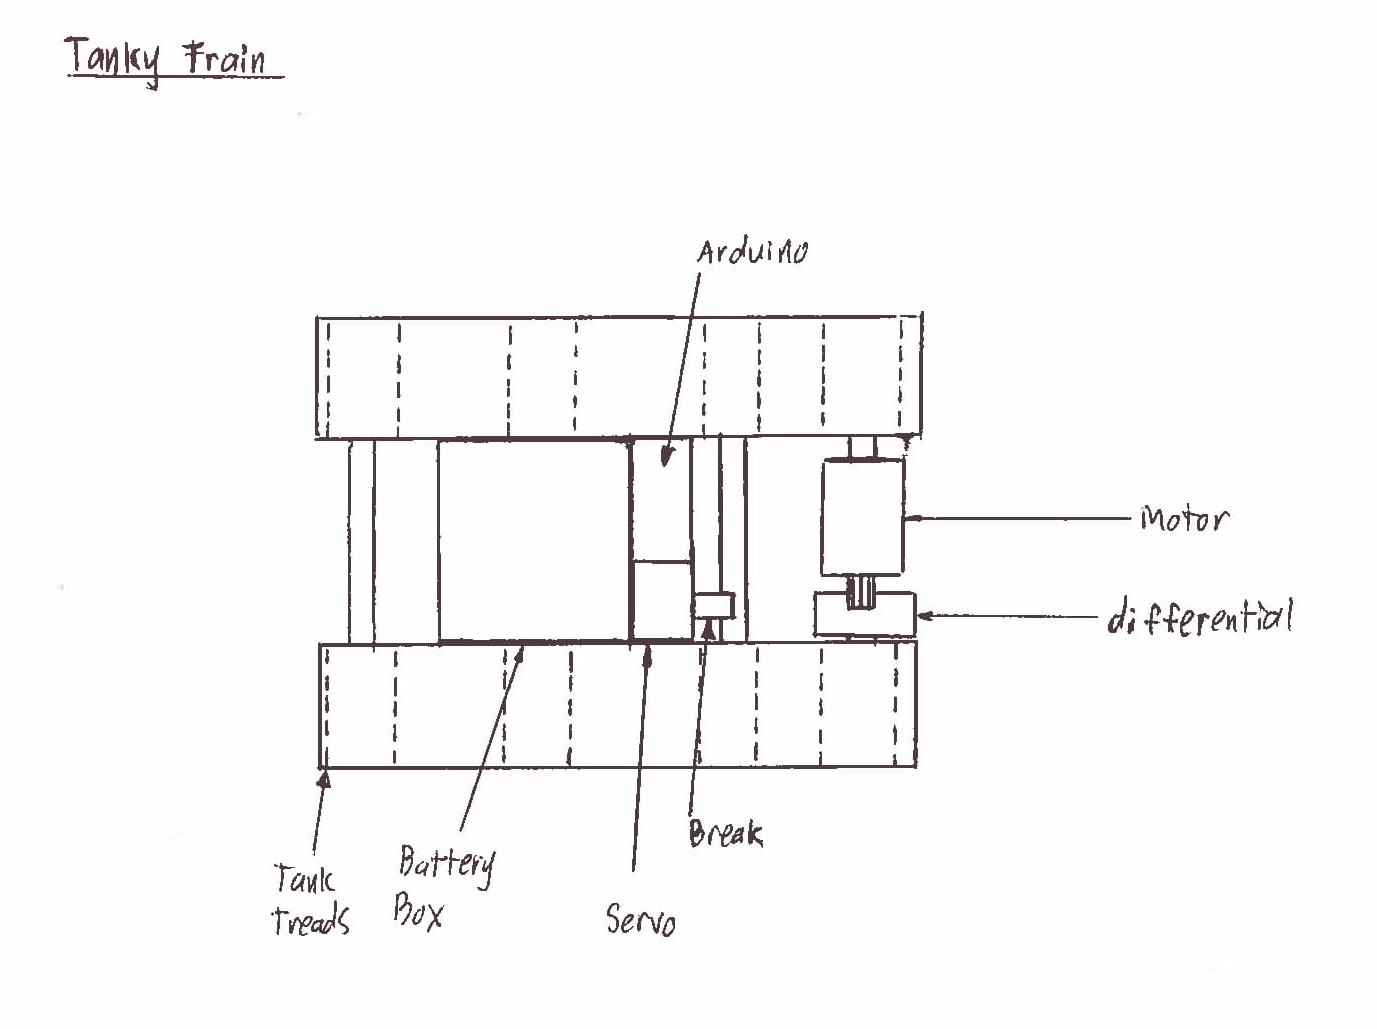
\includegraphics[width=0.8\textwidth]{../../res/img/tankytrain}
	\caption{Tanky Train Concept Sketch}
	\label{app/fig:tankytrain}
\end{figure}

Description: The motor directly drives the treads on the wheels.
A differential is used to give the vehicle better cornering.
A drum brake will decelerate the vehicle before turns.
\clearpage

\begin{figure}[H]
	\centering
	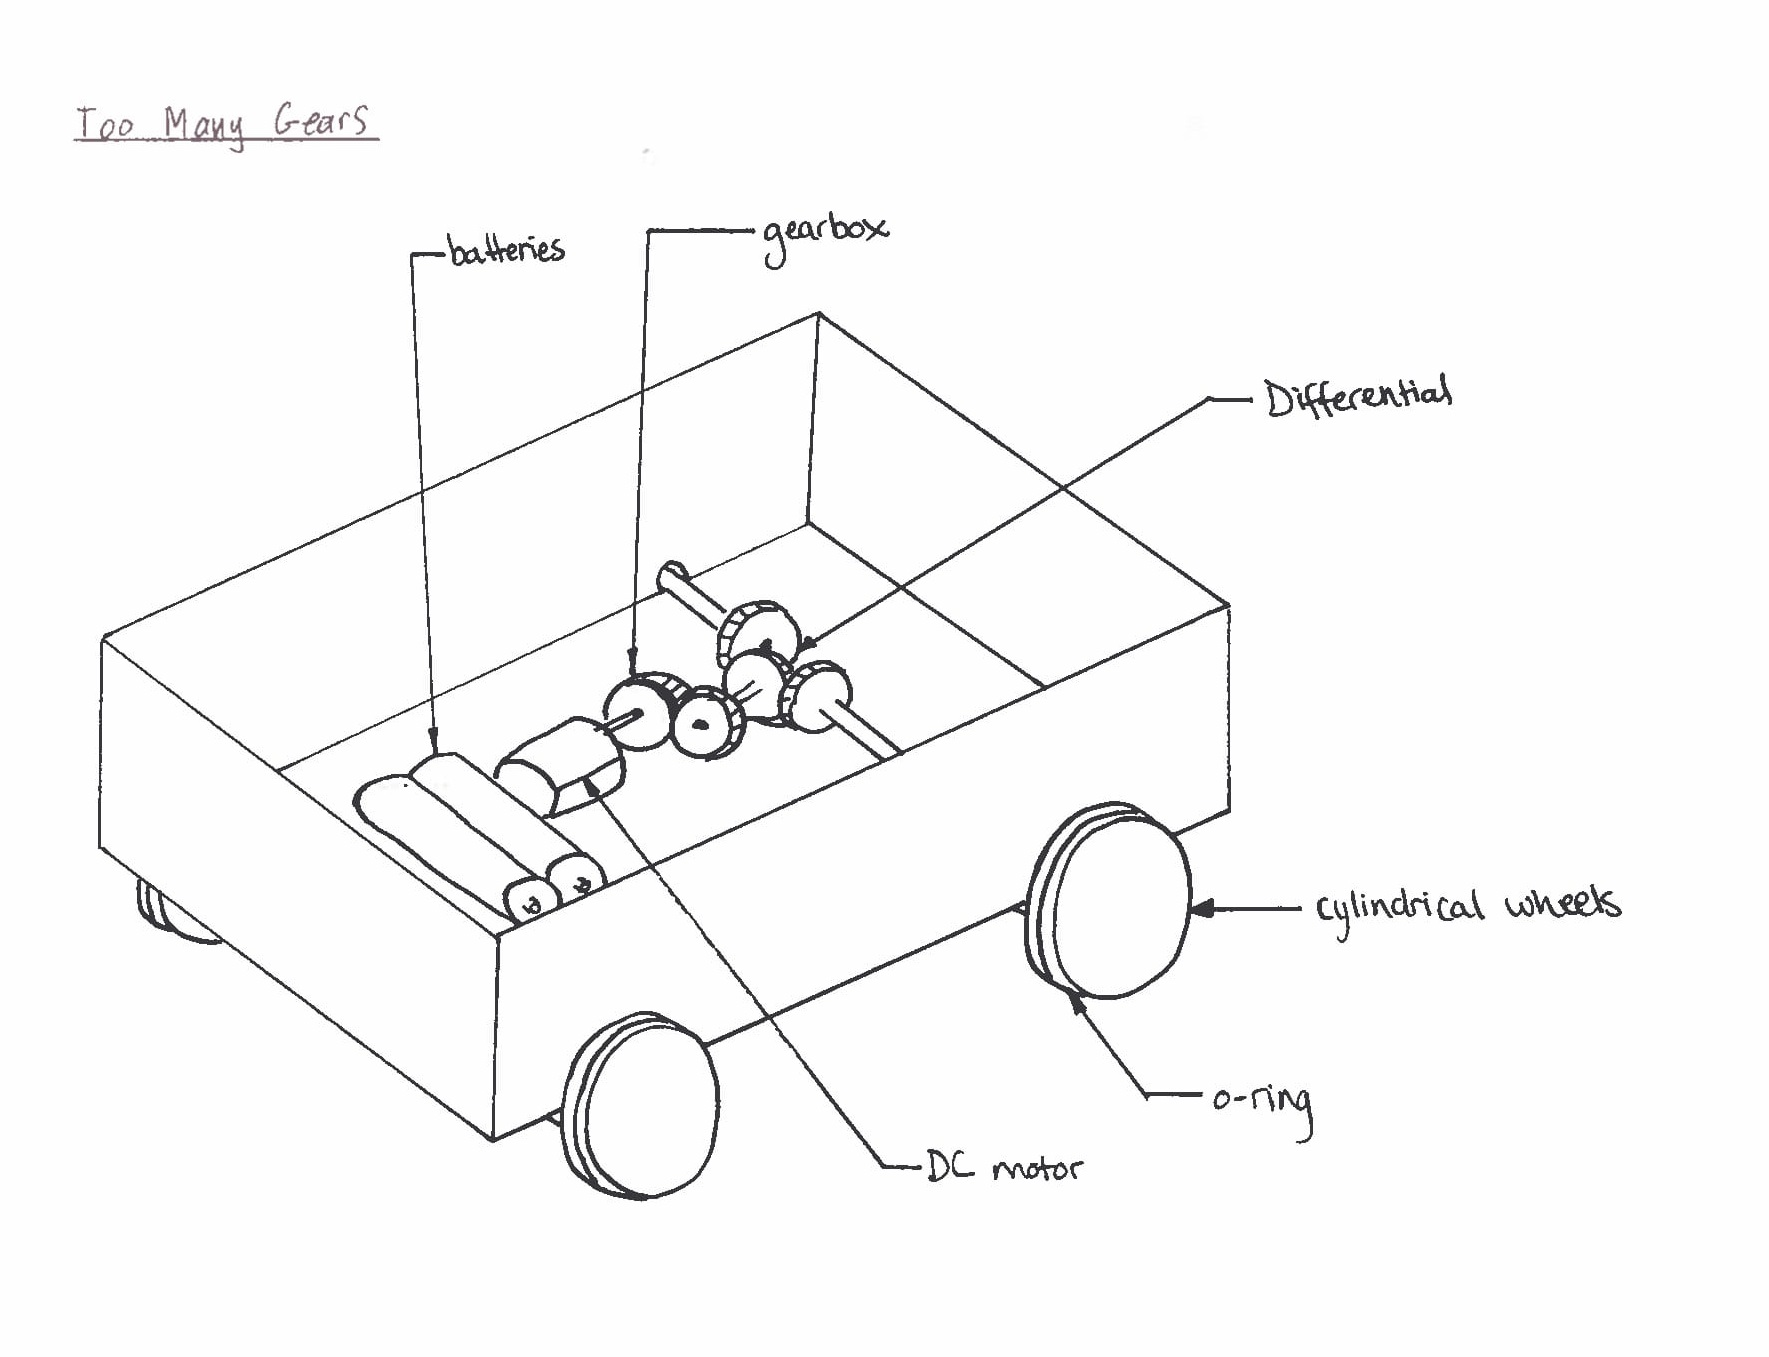
\includegraphics[width=0.8\textwidth]{../../res/img/tmg}
	\caption{Too Many Gears Concept Sketch}
	\label{app/fig:tmg}
\end{figure}

Description: Too Many Gears involves multiple gears to step down the speed.
The wheels have an o-ring to improve traction on a cylindrical surface.
This design also involves a slip differential to enable easier turning.
\clearpage

\begin{figure}[H]
	\centering
	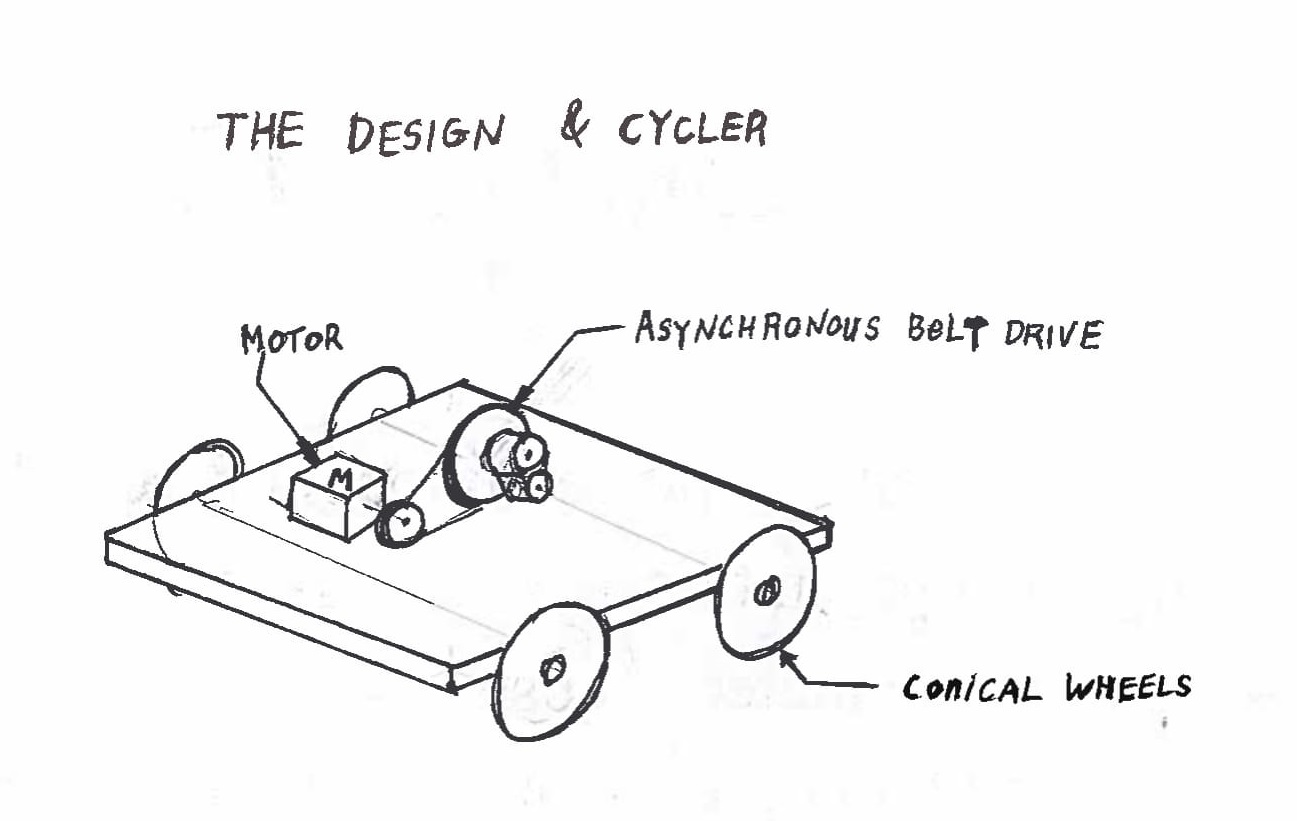
\includegraphics[width=0.8\textwidth]{../../res/img/designcycler}
	\caption{The Design Cycler Concept Sketch}
	\label{app/fig:designcycler}
\end{figure}

Description: The Design Cycler involves a multiple asynchronous belt drive mechanism that reduces the speed.
The motor is directly connected to the batteries and is controlled by a single switch, making this vehicle single speed.
Conical wheels enable smoother turning and better control.
\clearpage

\begin{figure}[H]
	\centering
	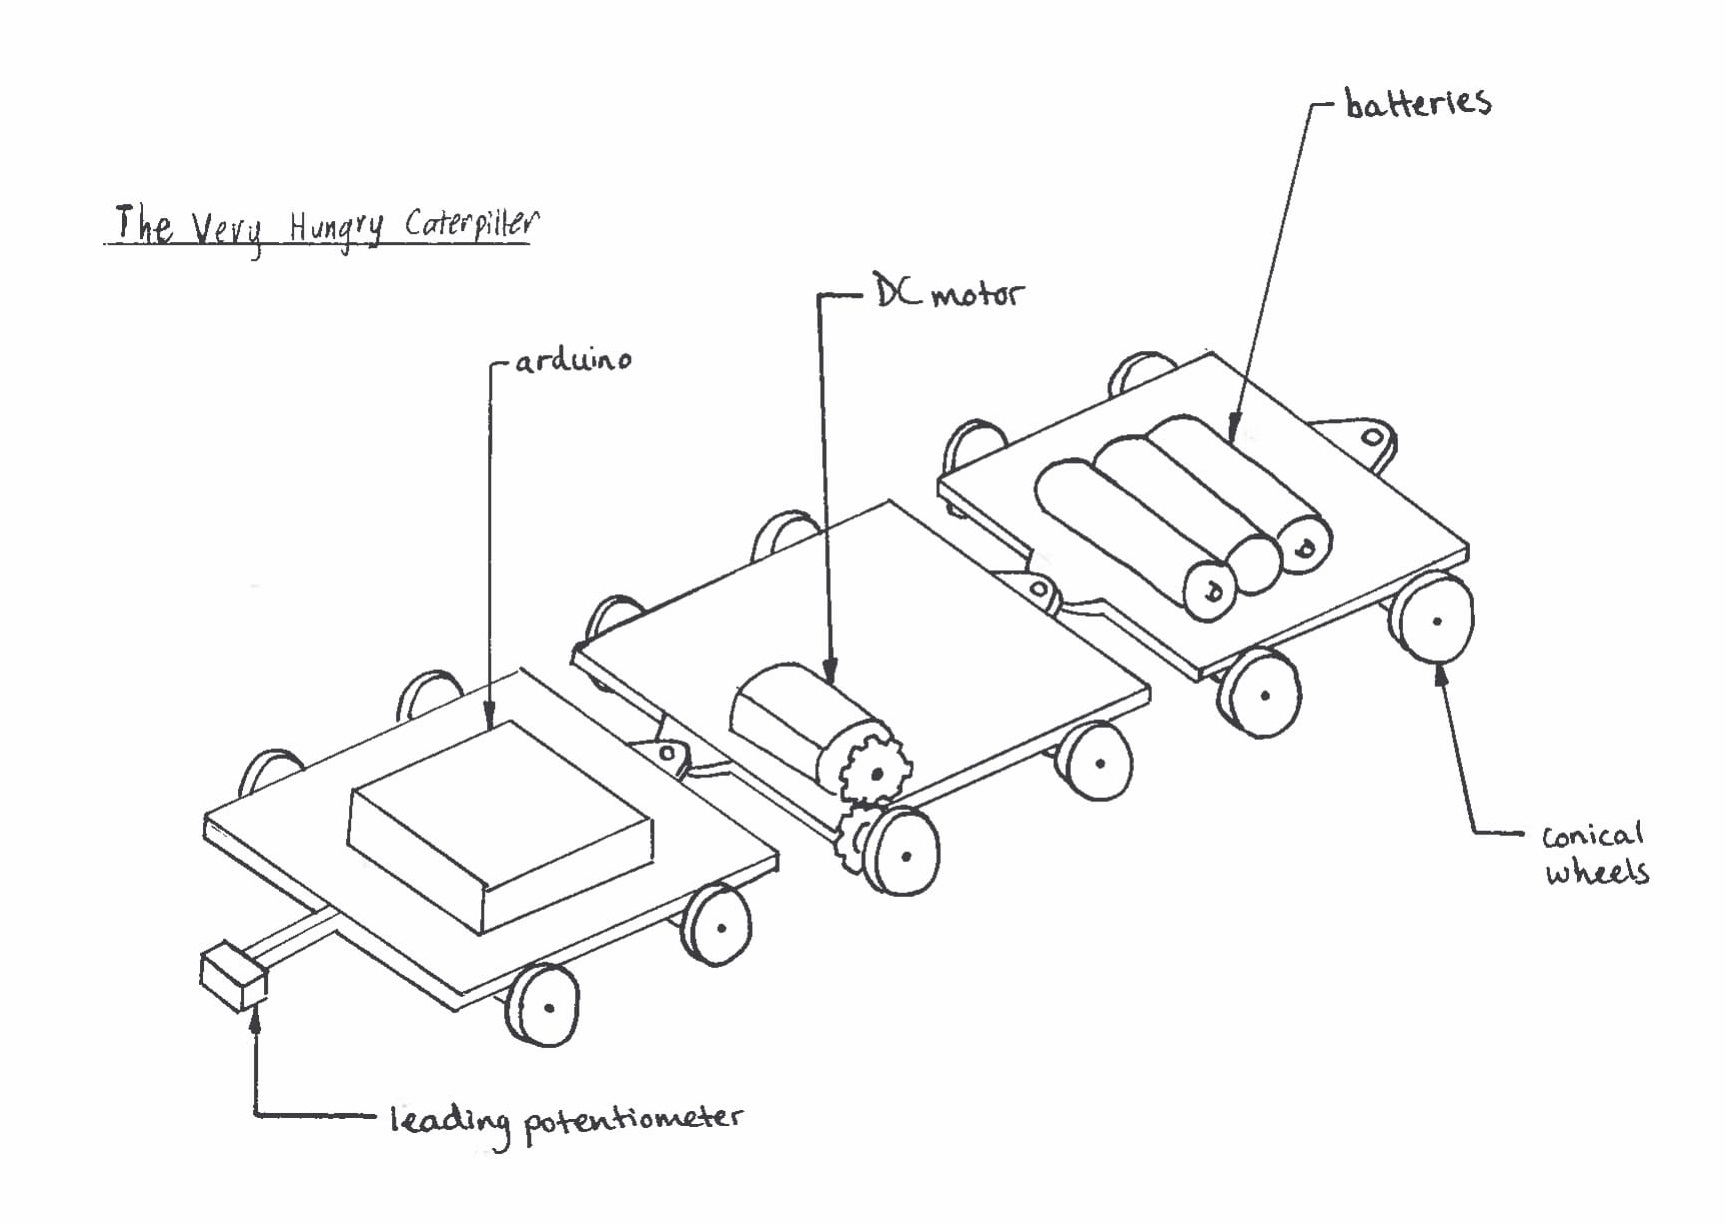
\includegraphics[width=0.8\textwidth]{../../res/img/tvhc}
	\caption{The Very Hungry Caterpillar Concept Sketch}
	\label{app/fig:tvhc}
\end{figure}

Description: The Very Hungry Caterpillar (TVHC) is a multiple car locomotive design.
Each car supports a different component; and the middle cart is directly driven by the DC motor.
This design involves a potentiometer coupled with an arduino to detect turns and slow down.
\clearpage

\begin{figure}[H]
	\centering
	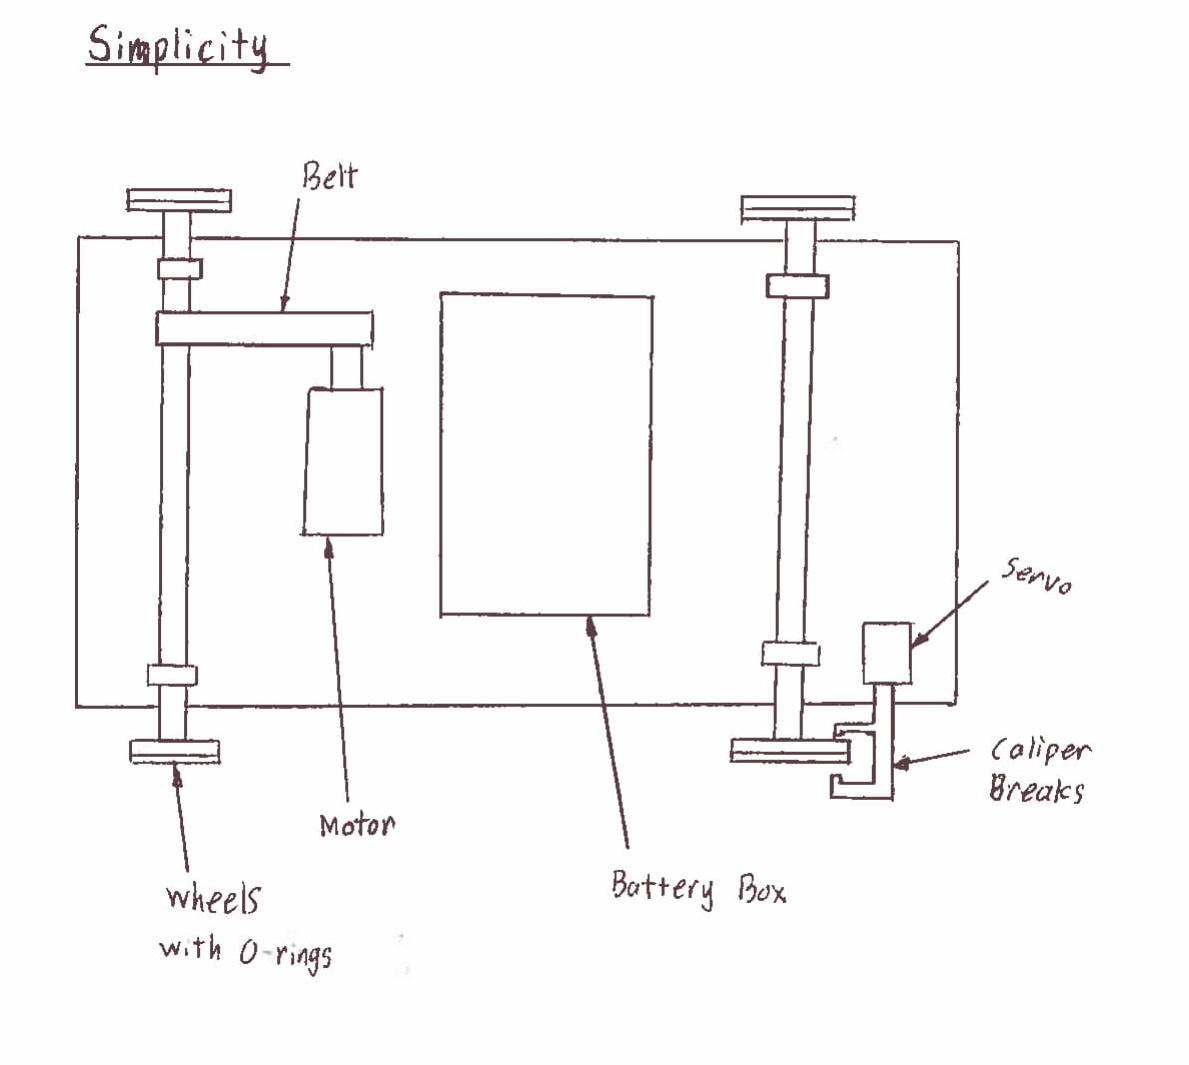
\includegraphics[width=0.8\textwidth]{../../res/img/simplicity}
	\caption{Simplicity Concept Sketch}
	\label{app/fig:simplicity}
\end{figure}

Description: Simplicity has relatively few components.
It uses a belt drive system and caliper brakes to control speed.
Wheels with o-rings allow for better cornering.
\clearpage

\begin{figure}[H]
	\centering
	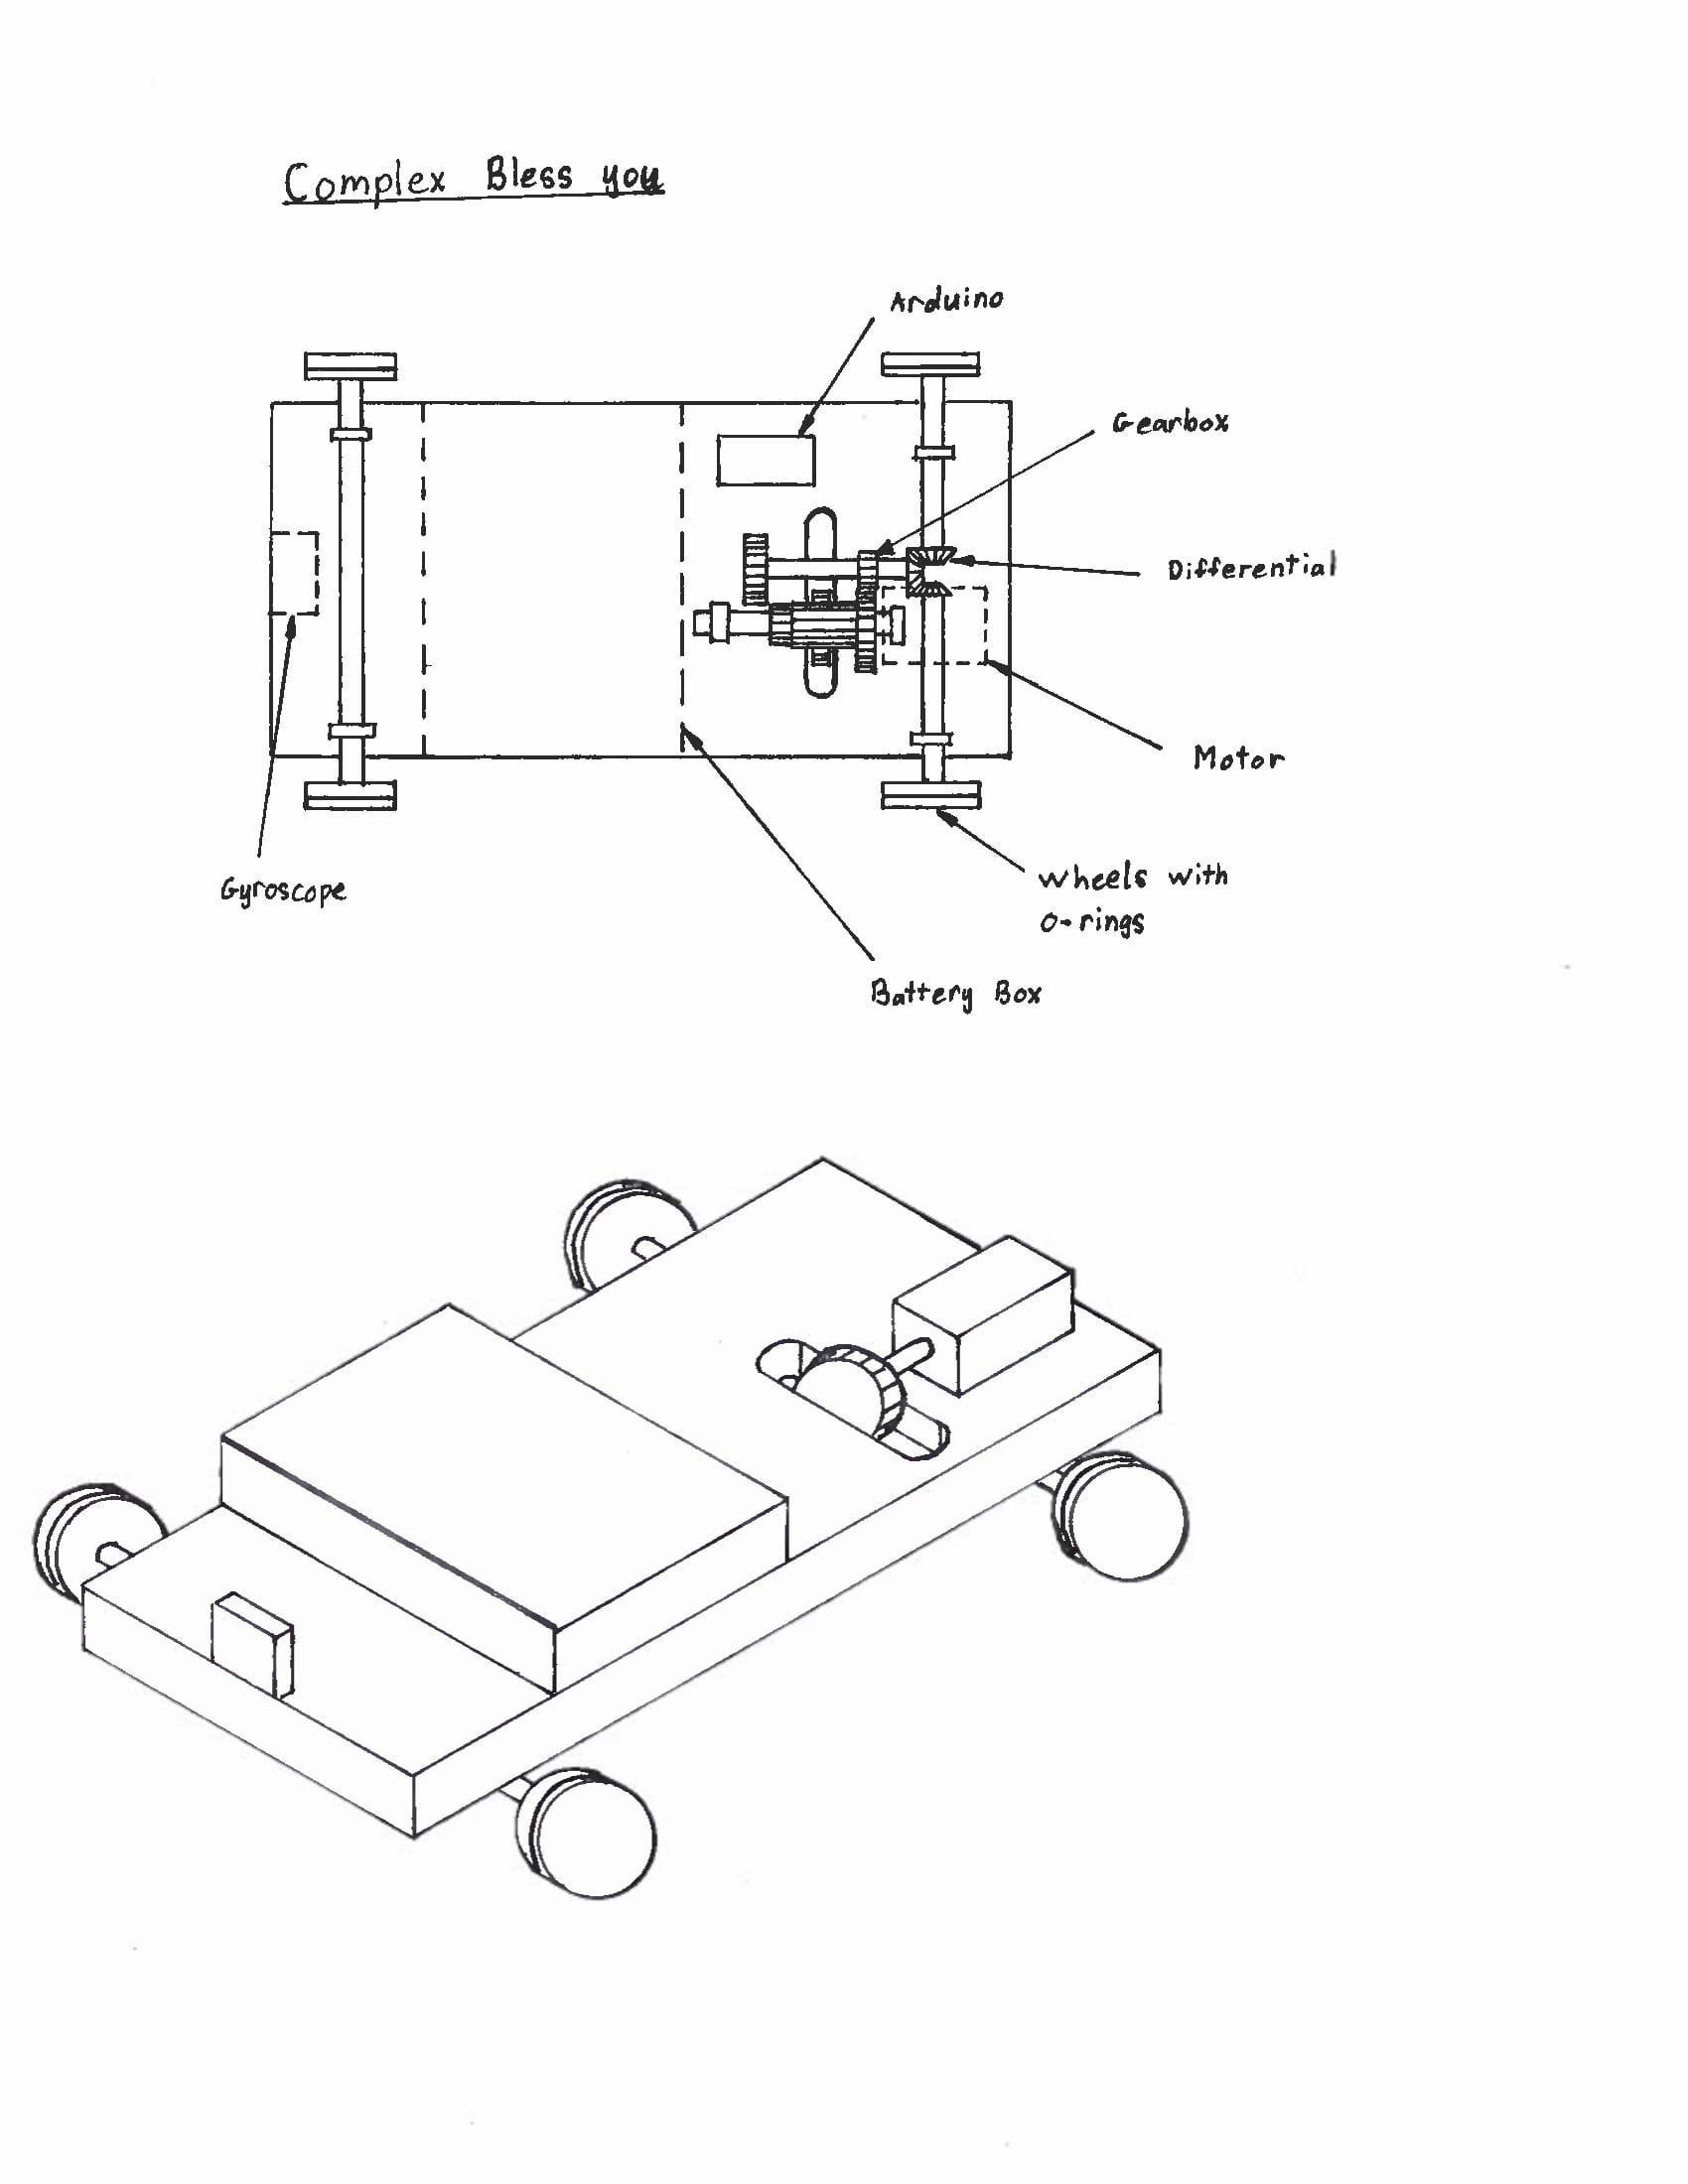
\includegraphics[width=0.8\textwidth]{../../res/img/cby}
	\caption{Complex Bless You}
	\label{app/fig:cby}
\end{figure}

Description: After noticing the similarity between multiple concepts, we combined them into a single, improved design.
Complex bless you is a combination of the above designs Complexity (Figure B3), Too Many Gears (Figure B9) and Bless You (Figure B2).
This design features a gyroscope to detect turns and an arduino to control the speed in the gearbox.
Wheels with o-rings and a slip differential allow for smooth turning.
The gearbox is dual speed and can be controlled by the arduino through the servo.

\end{document}
